\chapter{Results and Interpretation}

\section{Parameters and Nondimensionalization}

For most analyses, many of the parameters and results are non-dimensionalized. In
particular, instead of separate parameters for \(k_z\) and \(k_{xy}\), \(k_z\)
and \(k_{\textrm{eff}}\) are both normalized by \(k_{xy}\). Numerical
experiments verified that this is permissible, as numerical experiments with
different \(k_z\) and \(k_{xy}\) parameters but equivalent ratios
\(\fracflat{k_z}{k_{xy}}\) resulted in very similar ratios of
\(\fracflat{k_{\textrm{eff}}}{k_{xy}}\).

Angle is an exception. In this analysis, all angles are given as degrees from
the horizontal (\(xy\)) plane.

\section{Numerical vs. Analytical Predictions}

A 3-D plot of the numerical and analytical predictions may be seen in 
Figures \ref{fig:numvanal}. This plot shows that the two approaches to predicting measured conductivity
as a function of angle and anisotropy ratio have similar trends. However,
there are important disagreements which must be resolved.

\begin{figure}[h]
\centering
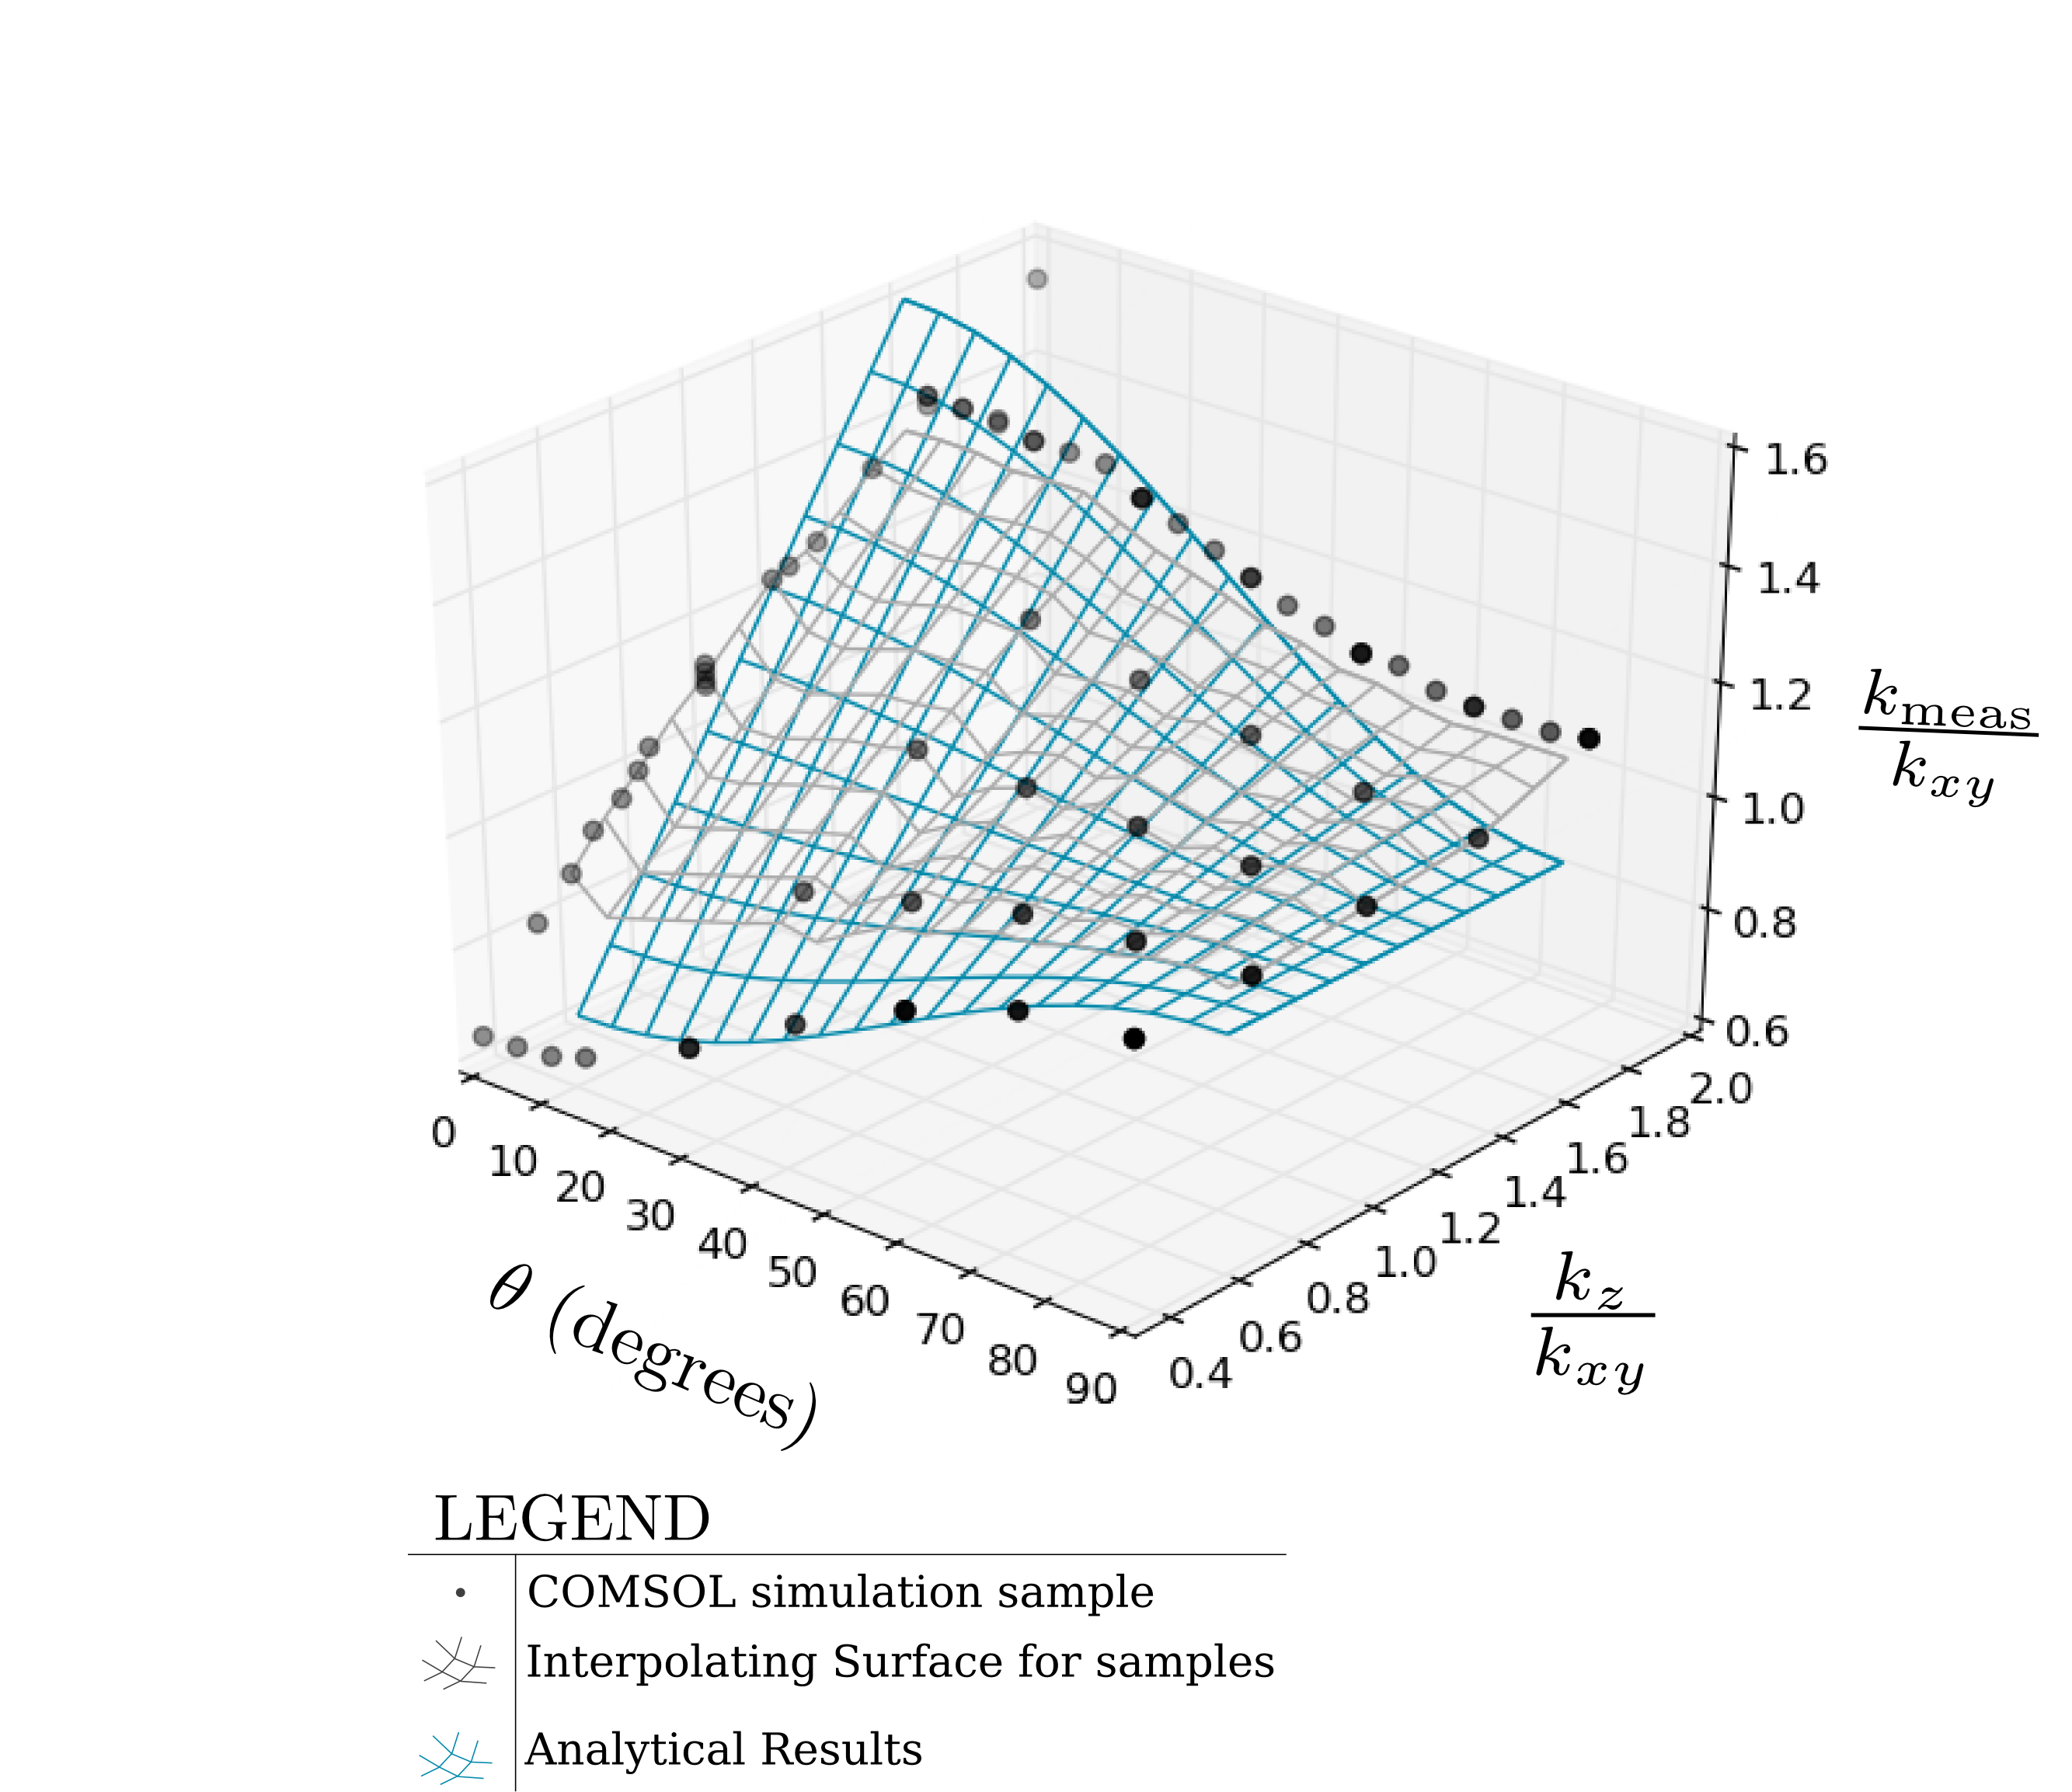
\includegraphics[width=\textwidth]{fig/numvanal.png}
\caption{A comparison of the numerical results and the analytical theory shows
general agreement. Grey dots represent numerical simulation results, the grey surface represents an interpolating surface of the dots, and the blue surface represents the analytical model. Disagreement between the two may be due to edge effects and/or numerical
model convergence issues.}
\label{fig:numvanal}
\end{figure}

Many details may be seen more readily in two-dimensional plots. In particular,
Figure \ref{fig:by_angle} shows theoretical predictions from both the analytical
and numerical model as a function of anisotropic conductivity ratios, sliced by
angle, while Figure \ref{fig:by_kratio} shows theoretical predictions from both
methods as a function of angle, sliced by anisotropic conductivity ratios.
Figure \ref{fig:by_angle} readily shows that an increase in conductivity ratio
above \(1\) has a weaker effect on effective conductivity for the numerical
model than in the analytical model. This may be due to edge effects decreasing
the effective thermal conductivity in the numerical model by conducting heat
axially from the needle. The analytical model, in contrast, does not model edge
effects, as it models an infinitely long needle like the
original needle probe method. For the isotropic case, these edge effects have
been studied and quantified analytically by other researchers. \cite{axialerror}

\begin{figure}[h]
\centering
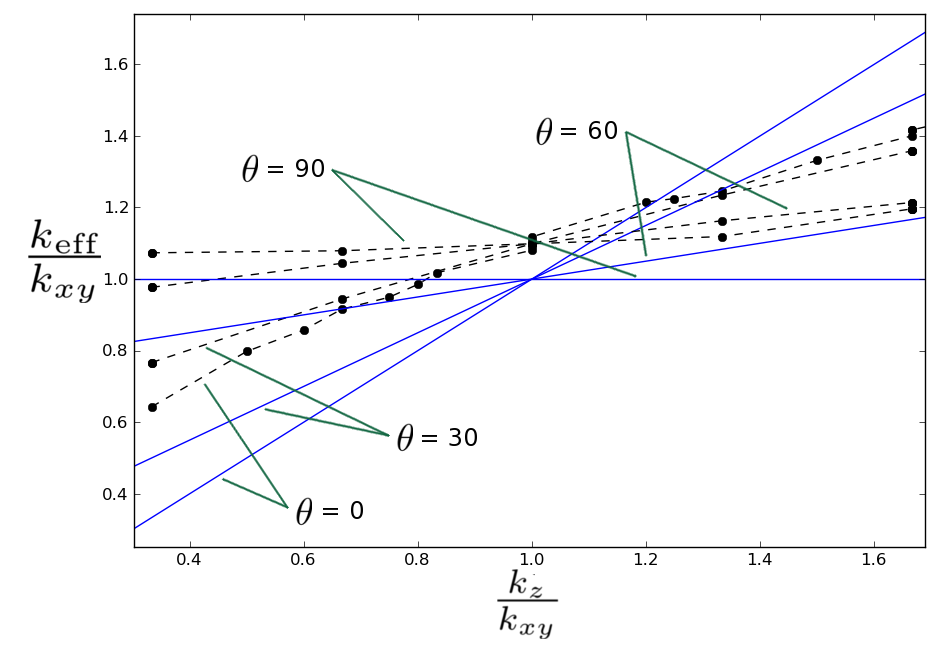
\includegraphics[width=0.8\textwidth]{fig/byAngle.png}
\caption{Slices of theoretical predictions by angle. Black points connected by dashed lines represent numerical results, while solid blue lines represent analytical theory. It can be seen that the analytical theory predicts measured conductivity to be a stronger function of angle than the numerical data at
higher conductivity ratios.}
\label{fig:by_angle}
\end{figure}

Figure \ref{fig:by_kratio} also shows the smoothing seen in Figure 
\ref{fig:by_angle}, but also readily shows the predictions of both models for
the isotropic case (\(\flatfrac{k_{\textrm{eff}}}{k_{xy}} = 1\)). Both models
correctly predict that effective thermal conductivity is not a function of angle
for the isotropic case. However, it is also clear that the numerical model
over-predicts \(k_{\textrm{eff}}\) by at least \(10\%\). Some of this may also
be due to edge effects, as evidenced by the cluster of points at the zero angle
(More readily seen in Figure \ref{fig:angle0}), where it can be seen that, in fact,
the predictions for the numerical method are a very weak function of \(k_{xy}\)
and not just the ratio of the anisotropic conductivities. 

\begin{figure}[h]
\centering
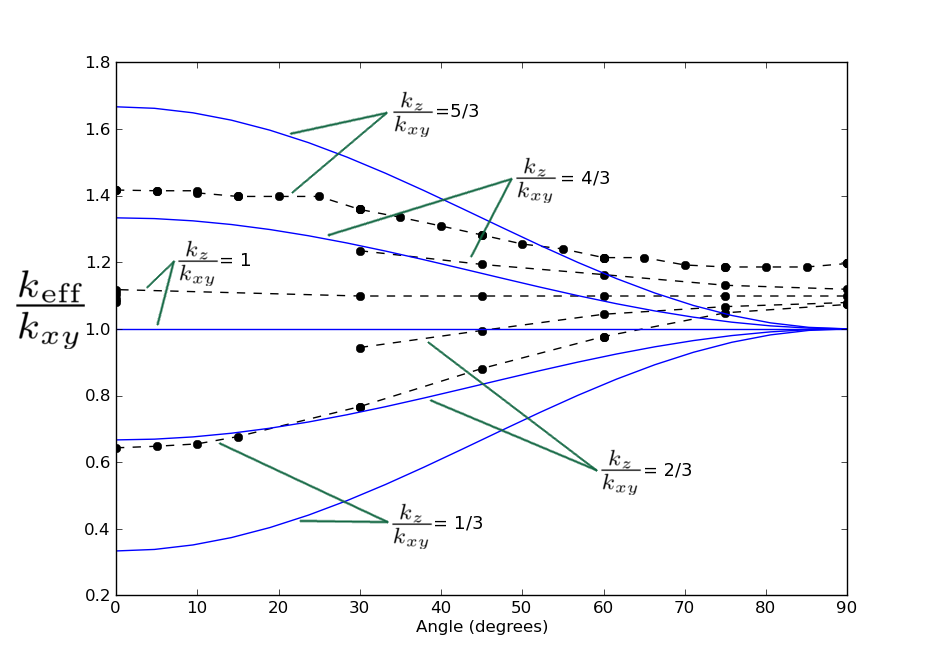
\includegraphics[width=0.8\textwidth]{fig/byKratio.png}
\caption{Slices of theoretical predictions by \(\flatfrac{k_z}{k_{xy}}\). Black points connected by dashed lines represent numerical results, while solid blue lines represent analytical theory. It can be seen that the analytical theory
is perfect for the isotropic case (\(\flatfrac{k_z}{k_{xy}} = 1\)), while the numerical experiments report larger-than-expected values.}
\label{fig:by_kratio}
\end{figure}

However, the dominant
cause for this discrepancy is believed to be due to using a model with too
coarse of a mesh. The convergence study results show that, while the time/temperature curves look
largely the same (Figure \ref{fig:conv_curves}), that the minor differences are magnified when taking the
derivative with respect to \(\ln(t)\) such that the coarse grid reports a
thermal conductivity of about \(110\%\) of the finer grid (Table \ref{tab:conv_kvals}).  This can be resolved in part with an extended convergence study.


\begin{figure}[h]
\centering
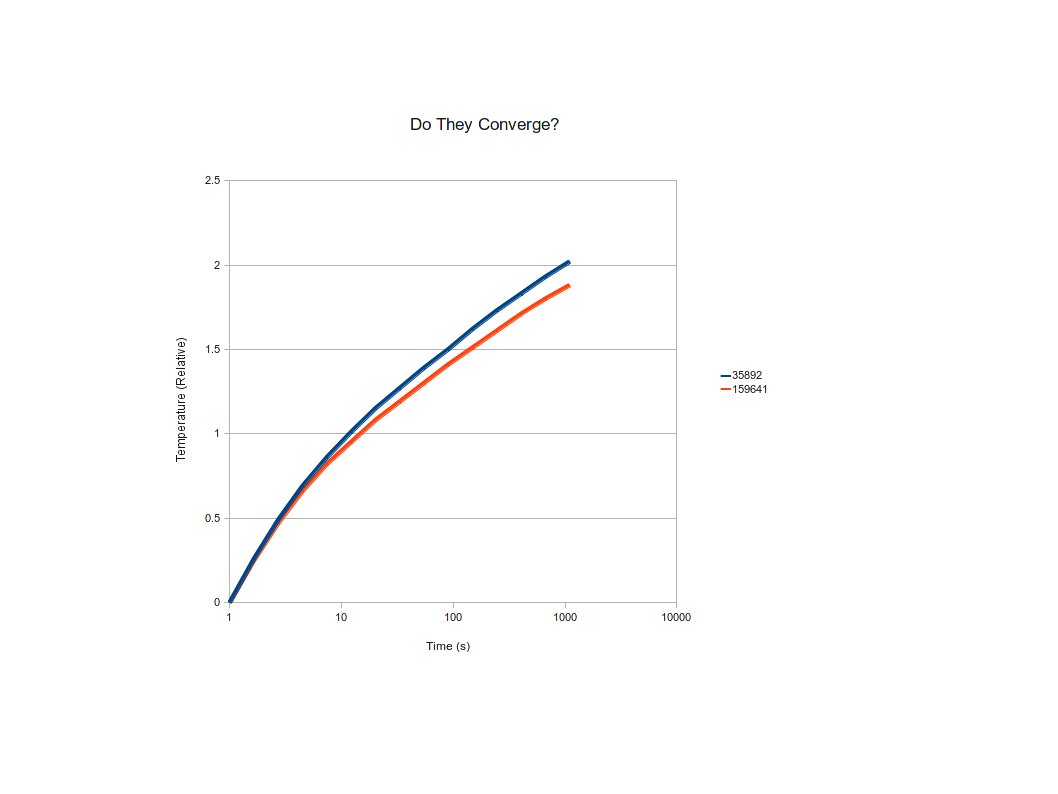
\includegraphics[width=0.6\textwidth]{fig/conv_curves.png}
\caption{A comparison of two \(T(t)\) curves from equivalent simulations with 
different fineness of mesh. These two curves appear quite similar, but their long-
time slopes are measurably different}
\label{fig:conv_curves}
\end{figure}


\begin{table}[h]
\centering
\begin{tabular}{r | l}
 & Slope\\
\(35892\) elements & 0.215\\
\(159641\) elements & 0.198\\
\% Error & 8.64 \%
\end{tabular}

\caption{A comparison of \(k_{\textrm{eff}}\) from two equivalent simulations 
with different fineness of mesh. Despite the similarities in time/temperature
curves, the resulting  conductivity calculations differ by nearly 10 \%. Units are in W\(/\)m\(\cdot\)K.}
\label{tab:conv_kvals}
\end{table}

Figure \ref{fig:angle0} shows predictions for the special case of
\(\theta = 0 \), where the needle is oriented parallel to the planes of isotropy.
This special case is of interest because previous needle probe measurements have
determined effective conductivities at this angle, which may or may not be
accurate representations of \(k_z\), the vertical thermal conductivity, which is
what is measured by a guarded hot plate apparatus and is the conductivity
of interest to climatologists modeling heat transfer between the atmosphere and
soil. If predictions for \(k_{\textrm{eff}}\) are \emph{equal} to \(k_z\), then
the measured \(k_{\textrm{eff}}\) accurately reflects \(k_z\). This agreement
between measurements seems unlikely for anisotropic measurements, and in fact 
the numerical model shows the expected trend of \(k_{\textrm{eff}} > k_z\) for
low conductivity ratios, and \(k_{\textrm{eff}} < k_z\) for higher conductivity
ratios. However, the analytical model predicts that \(k_{\textrm{eff}} = k_z\)
for all anisotropy ratios. While the analytical model shows expected behavior
for the isotropic case and shows the general trends one would expect, this
surprising result casts doubt onto the validity of the analytical model.

\begin{figure}[h]
\centering
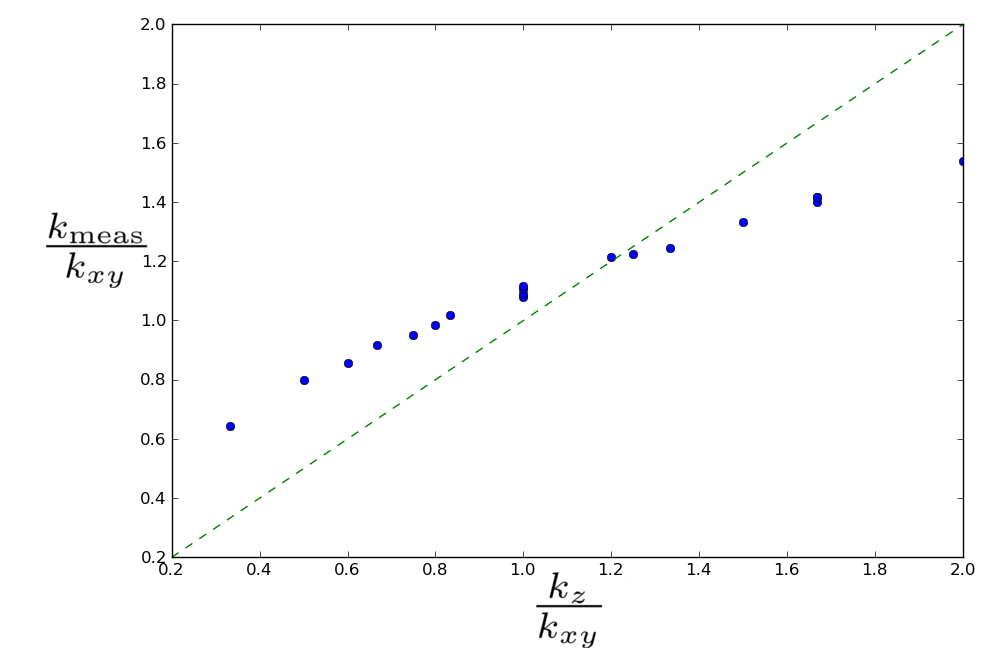
\includegraphics[width=0.8\textwidth]{fig/angle_0.png}
\caption{Theoretical predictions for the special case of \(\theta = 0 \),
when the needle is oriented horizontally. Blue points represent numerical solution, while green shows the line where \(k_{\textrm{eff}} = k_z\), where measured conductivity and vertical conductivity are the same. The analytical predictions are indistinguishable from this line, and are therefore not plotted.}
\label{fig:angle0}
\end{figure}


\section{Benchtop Measurements}

\begin{figure}[h]
\centering
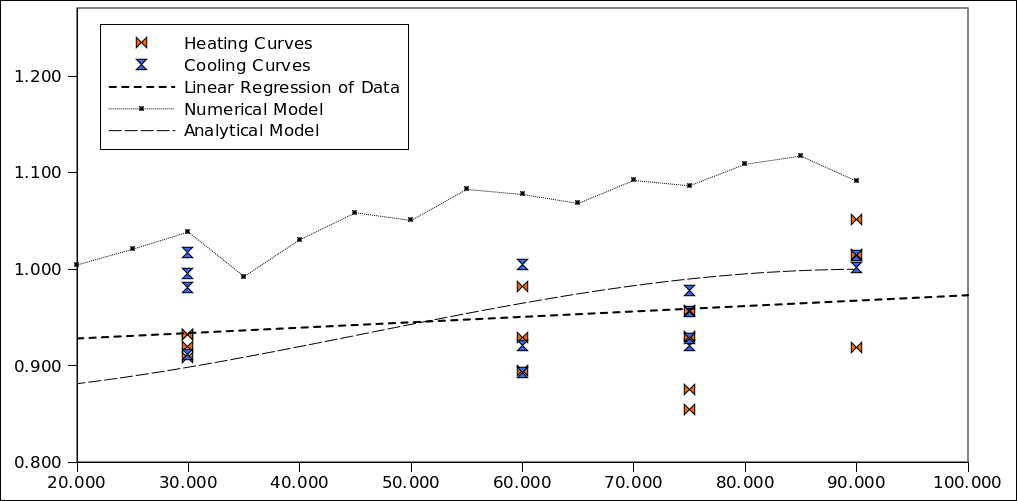
\includegraphics[width=0.9\textwidth]{fig/test_results.png}
\caption{A comparison of the benchtop measurements with the numerical and
analytical predictions for alternating layers of salt and sugar, given the
calculated anisotropic thermal conductivity.}
\label{fig:test_results}
\end{figure}

\begin{table}[h]
\centering
\begin{tabular}{l l | l l}
Angle (degrees) & # & Heating & Cooling\\
90 & 1 & 0.223284242942 & 0.243481576262\\
& 2 & 0.246684312618 & 0.24641641198\\
& 3 & 0.255505537961 & \sout{0.318256880271}\\
75 & 1 & 0.212791418373 & 0.223684883264\\
& 2 & 0.2325853424 & 0.232407779425\\
& 3 & 0.207604305022 & 0.225508200642\\
& 4 & 0.22608462065 & 0.237662896347\\
60 & 2 & 0.238543591267 & 0.244064408529\\
& 3 & 0.225850168518 & 0.22374914604\\
& 4 & 0.217518339596 & 0.216990054548\\
30 & 1 & 0.226573190917 & 0.238313150421\\
& 2 & 0.226429675463 & 0.247135960358\\
& 3 & 0.220619372302 & 0.241951060919\\
& 4 & 0.223387867071 & 0.221486604074\\
\end{tabular}

\caption{Raw data from the benchtop measurements. Note that one of the cooling curve measurements is striked out. This is because, when examined, it is clearly an outlier. Units are in W\(/\)m\(\cdot\)K.}
\label{tab:powders}
\end{table}


\begin{figure}[h]
\centering
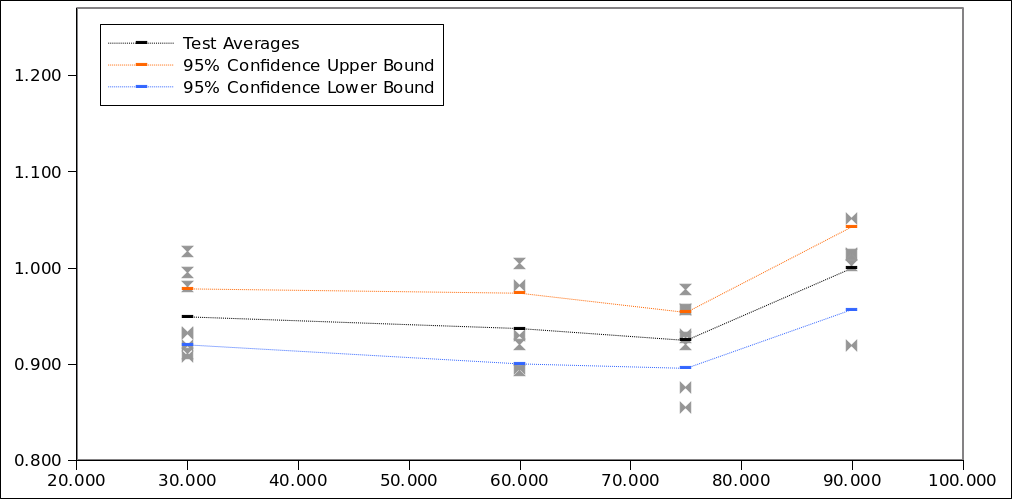
\includegraphics[width=0.9\textwidth]{fig/test_results_confidence.png}
\caption{Upper and lower bounds of 95 \% confidence in thermal conductivity measurements of the salt and sugar layered samples. This analysis 
indicates that the measurements can not statistically exclude a null hypothesis.}
\label{fig:test_confidence}
\end{figure}

\begin{table}[h]
\centering
\begin{tabular}{r | l l l}
 & \multicolumn{3}{c}{ \(k_{\textrm{meas}} / \bar{k_{xy}}\) }\\
Angle & Mean & Standard Deviation & 95\% Confidence\\
90 & 1.000 & 0.0491 & 0.0431\\
75 & 0.923 & 0.0419 & 0.0291\\
60 & 0.937 & 0.0459 & 0.0367\\
30 & 0.949 & 0.0420 & 0.0291\\
\end{tabular}

\caption{Basic statistics on normalized benchtop measurements.  Units are in W\(/\)m\(\cdot\)K.}
\label{tab:pow-stats}
\end{table}


It may be seen that there is a significant amount of variation between
benchtop measurements using the needle probe method in Figure \ref{fig:test_results} and Table \ref{tab:pow_stats}, even accounting for obviously failed measurements such as the removed outlier in Table \ref{tab:test_results}.
This is likely due in part to the nature of numerical derivatives as well as the relatively
unpredictable behavior of porous materials. Given
this variation, it is difficult to see which of the two models (analytical or numerical) is more appropriate.

Based on a general curve fit, the benchtop results show a slight upward slope (Figure \ref{fig:test_results}) as
expected. However, given the variation in the benchtop results, it is statistically
possible that angle has absolutely no effect on the reading. This could be fixed
with more careful, exacting standards in the construction of the anisotropic
materials, more measurements at each angle, and measurements at more angles.
In other words, given the variance of the measurements, many more measurements
would have to be made in order to reach any statistically significant
conclusions, at least given the relatively low amount of anisotropy of the sample.

Also given this variation and the relatively weak levels of anisotropy in the
sample, even with more measurements it could still prove difficult to deduce
the degree of anisotropy of the sample with this data and a curve fit to either
the numerical or analytical predictions alone.

\section{In-Situ Snow Measurements}

% This would be a good thing for an appendix.
\begin{comment}
\begin{table}[h]
\centering
\begin{tabular}{l | l l}
\# & h (inches) & Angle (degrees)
5 & 10.5 & 85\\
6 & 10.5 & 85\\
7 & 13 & 38\\
8 & 12.5 & 45\\
9 & 10.5 & 92
\end{tabular}

\label{tab:metadata}
\caption{Height and angle measurements from snow measurements. The height data was unused in this analysis.}
\end{table}
\end{comment}

\begin{table}[h]
\centering
\begin{tabular}{r | l l}
Angle & Heating & Cooling\\
0 & 0.0289 & 0.0321\\
5 & 0.0269 & 0.0244\\
45 & 0.0290 & 0.0327\\
52 & 0.0288 & 0.0326\\
\end{tabular}

\caption{Conductivity results from the snow measurements. Units are in W\(/\)m\(\cdot\)K.}
\label{tab:snow}
\end{table}

\begin{table}[h]
\centering
\begin{tabular}{r | l}
Control Volume & \(736.76\) mL\\
Mass & \(161.14\) g\\
Density & \(0.219\) g/mL\\
& 219 kg/\(\textrm{m}^3\)\\
\end{tabular}

\caption{Measured and derived measurements for snow density. Units are in W\(/\)m\(\cdot\)K.}
\label{tab:density}
\end{table}

\begin{figure}[h]
\centering
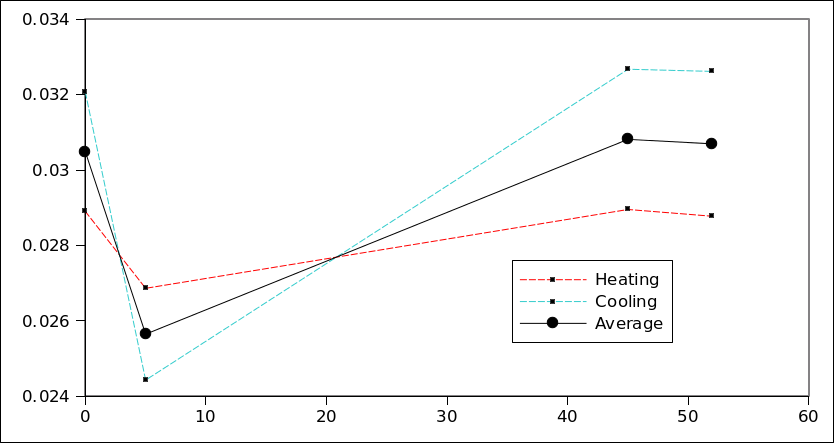
\includegraphics[width=0.9\textwidth]{fig/snow_meas.png}
\caption{Conductivity measurements in roughly the same layer of snow at various 
angles. Even a limited amount of in-situ snow measurements suggest a degree of
anisotropy.}
\label{fig:snow_results}
\end{figure}

\begin{figure}[h]
\centering
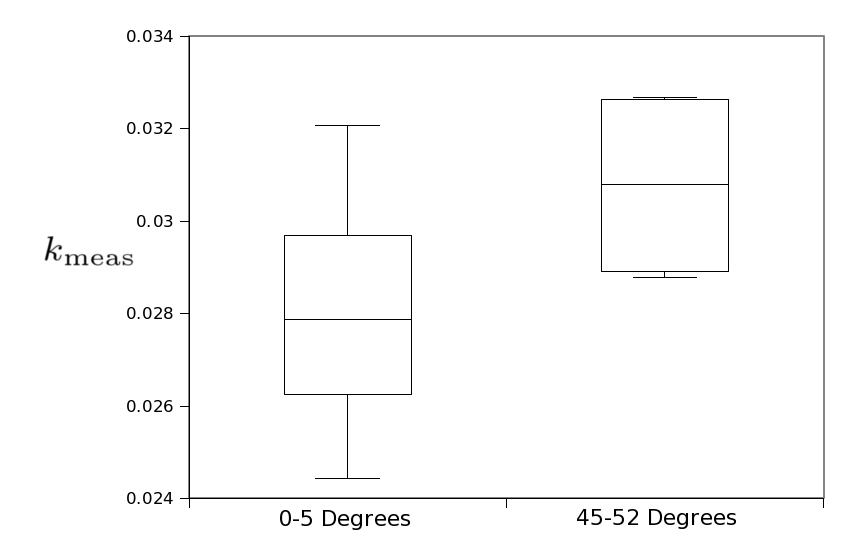
\includegraphics[width=0.9\textwidth]{fig/snow_meas_boxplot.png}
\caption{These boxplots give a general idea of the differences in measurements
between the near-horizontal angle and the more oblique ones in snow.}
\label{fig:test_boxplot}
\end{figure}


Due to the difficulty in taking snow measurements, very few snow measurements were
successfully completed (Table \ref{tab:snow}). This, on top of the inherent variation between measurements seen in the method, snow measurements are also inconclusive. However, the
measurements taken \emph{do} indicate anisotropy to a greater degree of confidence
than the benchtop measurements, as may be seen in Figures \ref{fig:snow_results}
 and \ref{fig:test_boxplot}. Like the case of the benchtop measurements, with so few
measurements a curve fit against either method of prediction is unlikely to
yield useful results.

To put the snow measurements in context for comparison in future studies, Table
\ref{tab:density} shows the snow density in the region of snow
that these measurements were taken.
